L'objectif de cette section est de comprendre et expérimenter la génération de différents types d'ondes dans un solide isotrope.

Dans la suite plusieurs manipulations sont réalisées :

\begin{itemize}
    \item mesures en mode écho \& mesure de la vitesse des ondes longitudinales (A-Scan)
    \item mesures en transmission \& évaluation de l'influence de l'angle d'incidence
    \item mesures de la vitesse d'ondes de surface en mode écho et transmission latérale
    \item mesures du re-rayonnement associé à la propagation d'une onde de Rayleigh généralisée\footnote{\textit{Leaky Rayleigh Wave}}
\end{itemize}

\section{Analyse théorique}

\label{volsurf:theo}

En premier lieu, il convient d'examiner les différents angles critiques à l'interface plexiglas/aluminium. Les paramètres des deux matériaux sont regroupés en table~\ref{volsurf:params}.

\begin{table*}[h]
    \centering
    \begin{tabular}{l|cc}
        Paramètre & Valeur & Unité\\\hline
        Vitesse de l'onde longitudinale dans l'aluminium $v_L$ & $6450$ & $m.s^{-1}$\\
        Vitesse de l'onde transversale dans l'aluminium $v_T$ & $3100$ & $m.s^{-1}$\\
        Vitesse de l'onde longitudinale dans le plexiglas $\tilde{v_L}$ & $2700$ & $m.s^{-1}$\\
        Vitesse de l'onde transversale dans le plexiglas $\tilde{v_T}$ & $1100$ & $m.s^{-1}$\\
        Épaisseur de la plaque $e$ & $20\cdot 10^{-3} \pm 0.1\cdot 10^{-3}$ & $m$\\
    \end{tabular}
    \caption{Paramètres remarquables de la manipulation.}
    \label{volsurf:params}
\end{table*}

\subsection{Angles Critiques}

D'après la loi de Snell-Descartes~\eqref{volsurf:snell}, viennent les calculs des angles incidents critiques (pour lesquels l'angle réfracté vaut 90\degre) en équations~\eqref{volsurf:Lcrit} &~\eqref{volsurf:Tcrit}.

\begin{equation}
    \frac{\sin \theta_1}{v_1} = \frac{\sin\theta_2}{v_2} \label{volsurf:snell}
\end{equation}

\begin{equation}
    \theta_{L_crit} = \arcsin\frac{\tilde{v_L}}{v_L} \overset{AN}{\approx} 24.7\deg \label{volsurf:Lcrit}
\end{equation}

\begin{equation}
    \theta_{T_crit} = \arcsin\frac{\tilde{v_L}}{v_T} \overset{AN}{\approx} 60.6\deg \label{volsurf:Tcrit}
\end{equation}

Les ondes se propageant dans une couche solide (aluminium) entre deux milieux solides de même nature (sabot en plexiglas), les calculs montrent que l'angle de sortie sera le même que l'angle d'entrée.

Pour optimiser la réception, il est judicieux d'orienter le transducteur de réception de manière analogue à celui d'émission. Il pourra également être nécessaire de décaler légèrement les transducteurs l'un par rapport à l'autre afin de bien centrer la réception sur le point d'émergence du faisceau en sortie de la couche métallique.

\subsection{Angle de Rayleigh}
\label{volsurf:theo:rayleigh_angle}

Les ondes de Rayleigh sont des ondes de surface se propageant à une vitesse inférieure à celle de l'onde transversale. 

Leur intérêt principal dans le cas du CND est la détection de défauts subsurfaciques où elles excellent à contrôler une zone souvent masquée dans le cadre d'autres méthodes (zone morte).

\paragraph{Équation de Rayleigh} En introduisant les nombres adimensionnels $\xi = \nicefrac{v_T}{v_L}$ et $\eta = \frac{v_R}{v_T}$ (où $v_R$ est la vitesse de propagation des ondes de Rayleigh), l'équation de Rayleigh s'exprime telle qu'en ~\eqref{volsurf:rayleigh_eq}.

\begin{equation}
    \eta^6 - 8\eta^4 + 8\eta^2(3-2\xi)^2 + 16(\xi^2-1) = 0 \label{volsurf:rayleigh_eq}.
\end{equation}

La solution approchée la plus utilisée pour déterminer la vitesse de propagation des ondes
de Rayleigh, dénommée solution de Viktorov~\autocite{viktorov_rayleigh_1970}), est proposée en~\eqref{volsurf:viktorov}.

\begin{equation}
    \eta = \frac{0.718 - \xi^2}{0.75 - \xi^2} \label{volsurf:viktorov}
\end{equation}

Il vient alors, compte-tenu des paramètres du problème présenté en table~\ref{volsurf:params} :

\begin{equation}
    v_R = v_T\frac{0.718-\xi^2}{0.75-\xi^2} \overset{AN}{\approx} = 2908 m\cdot s^{-1} \label{volsurf:an_viktorov}
\end{equation}

\paragraph{Angle de Rayleigh} Connaissant la vitesse de propagation des ondes de Rayleigh et sachant qu'il s'agit d'ondes de surface (angle réfracté valant 90\degres), il est possible de calculer l'angle d'incident optimal pour générer des ondes de Rayleigh. Toujours en utilisant la relation~\eqref{volsurf:snell} il vient :

\begin{equation}
    \theta_{R} = \arcsin\frac{\tilde{v_L}}{v_R} \overset{AN}{\approx} 68.2\deg \label{volsurf:thetaR}
\end{equation}

Comme dans une vaste majorité des cas, l'angle de Rayleigh $\theta_R$ est légèrement supérieur au deuxième angle critique.

\section{Onde de volume}

\label{volsurf:vol}

L'objet de l'étude expérimentale est ici la vérification des assertions suivantes :

\begin{enumerate}
    \item il n'y a plus d'onde longitudinale transmise après le premier angle critique ;
    \item il n'y a plus d'onde transversale transmise après le second angle critique ;
    \item le matériau est isotrope, la vitesse de propagation ne dépend pas de l'angle de propagation.
\end{enumerate}

\begin{figure*}
    \centering
    \begin{tikzpicture}
    \newcommand\transwedge[1]{
        \draw[thick, fill=white] (0,0) -- ++(4,0) -- (0,4) --cycle;
        \begin{scope}[shift={(0,-.3)}, rotate around={-#1:(3.4,0)}]
            \draw[thick] (2.5,3.6) -- ++(1.8,0) -- ++(0,-1) -- ++(-1.8,0) --cycle; % moving part
            \draw[thick] (2.5,3.6) rectangle ++(1.8,1.4); % tranducer
            \draw[thick] (3.4,5) .. controls (3.2,5.5) and (3.6,5.5) .. (3.4,6); % cable
        \end{scope}
        \draw[thick, fill=white] (.4,0) -- (6.4,0) arc (0:180:3); % half circle
        \foreach \i in {0,45,60,70}{
            \begin{scope}[rotate around={-\i:(3.6,.7)}]
                \draw (3.4,.3) -- ++(0,2);
            \end{scope}
        }
    }
    
    % part
    \draw[very thick] (-7,0) -- (7,0);
    \draw[very thick] (-7,-2) -- (7,-2);
    \draw[very thick] (-7,0) .. controls (-8,-1) and (-6,-1) .. (-7,-2);
    \draw[very thick] (7,0) -- ++(0,-2);
    %\begin{scope}[shift={(14,0)}]
    %    \draw[very thick] (-7,0) .. controls (-8,-1) and (-6,-1) .. (-7,-2);
    %\end{scope}
    
    \draw[<->, >=stealth] (7.3,0) -- ++(0,-2) node[midway, right, shift={(.3,1)}, rotate=-90] {$h=20mm$};
    
    % tranducers
    \begin{scope}[shift={(-6,0)}, scale=.3, transform shape]
        \transwedge{0}
    \end{scope}
    \draw (-5,2) node[above] {a) Mode écho};
    
    
    \begin{scope}[shift={(-1,0)}, scale=.3, transform shape]
        \transwedge{30}
    \end{scope}
    \begin{scope}[shift={(-1,0)}, yscale=-1, xscale=-1, shift={(-1,2)}, scale=.3, transform shape]
        \transwedge{30}
    \end{scope}
    \draw (0,2) node[above] {b) Mode transmission};
    
    
    \begin{scope}[shift={(6,0)}, xscale=-1, scale=.3, transform shape]
        \transwedge{60}
    \end{scope}
    \draw (5,2) node[above] {c) Ondes de Rayleigh};
    
    \end{tikzpicture}
    \caption{Différents montages expérimentaux utilisés. A gauche, en mode écho, l'onde est transmise en incidence normale et renvoyée par le fond de plaque. Au centre, en mode transmission, l'onde est transmise avec une incidence $\theta_I$ et est transmise avec le même angle en sortie de plaque. À droite, le mode écho est utilisée pour la détection d'onde de Rayleigh après leur réflexion en bord de plaque.}
    \label{volsurf:montages}
\end{figure*}

\subsection{Mode écho}
\label{volsurf:vol_echo}

L'objectif ici est de comparer la vitesse théorique de l'onde de compression avec sa vitesse effective.
Le montage expérimental utilisé est la configuration a) de la figure~\ref{volsurf:montages}.
Le transducteur émet une onde longitudinale se propageant dans le plexiglas puis arrivant avec une indidence normale sur l'interface plexiglas/aluminium.
Une onde longitudinale est alors générée dans l'aluminium et réfléchie sur le fond de plaque avant de revenir au transducteur.

A l'oscillocope, les temps de vol mesurées comprendrons donc deux fois le temps de vol dans les $h_w = 3.5cm$ de plexiglas qui séparent le transducteur de la plaque ainsi que 2 fois le temps de parcours de la plaque (aller-retour).

\begin{figurehere}
    \centering
    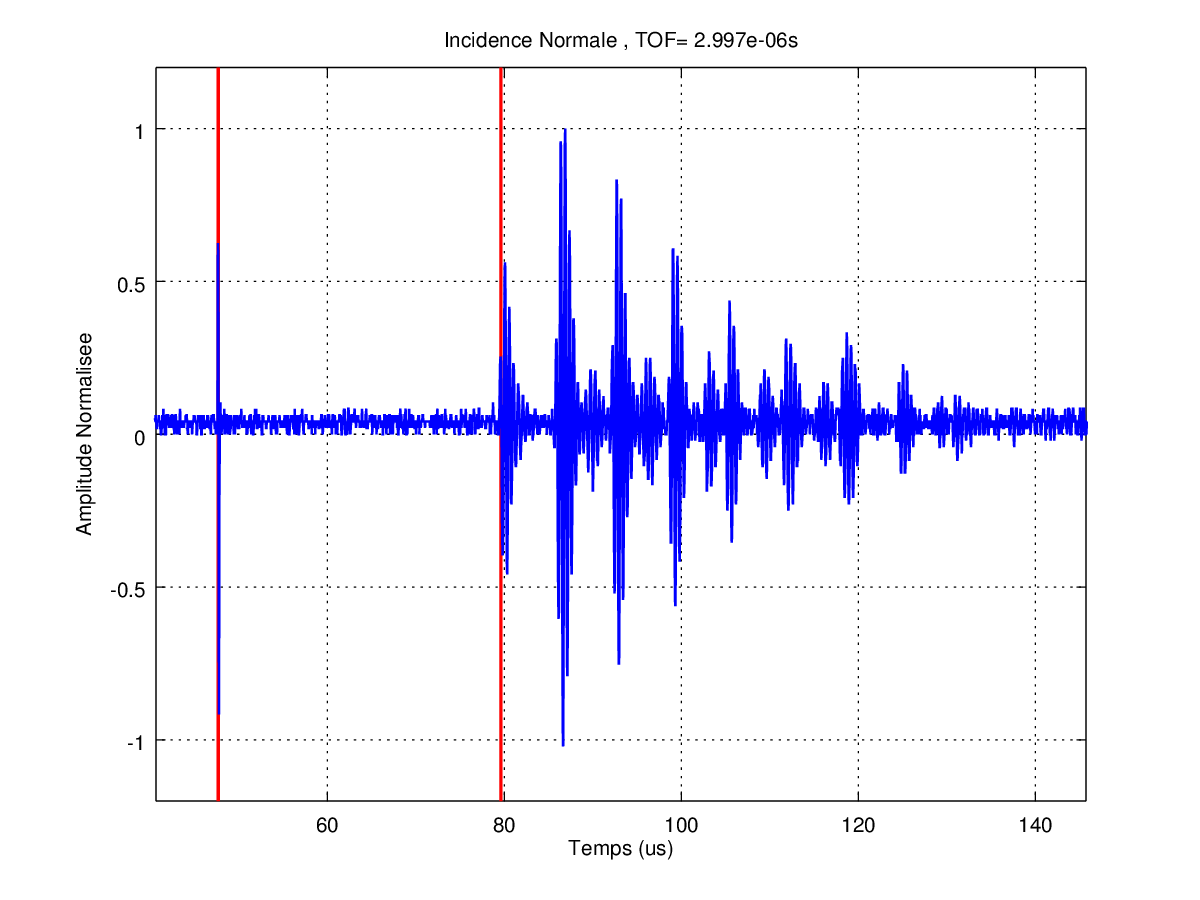
\includegraphics[width=.5\textwidth]{volsurf_figs/DS0000_incnorm.png}
    \caption{Mesure ultrasonore en mode écho. Connaissant l'écart temporel entre le signal de synchronisation (à environ $20\mu s$) et le début du premier écho (à environ $80\mu s$) il est possible de remonter à l'épaisseur de plaque (connaissant la vitesse ou \textit{vice versa}). Les calculs sont donnés au paragraphe~\ref{volsurf:vol_echo}.}
    \label{volsurf:echo_norm}
\end{figurehere}

La formule pour remonter à une estimation $\hat{v}_L$ de la vitesse des ondes longitudinales (seules excitées en incidence normale) est donnée en~\eqref{volsurf:back_to_longi} (où $\tau$ est le temps de vol relevé et $h$ l'épaisseur de la plaque). 

\begin{equation}
    \hat{v}_L = \frac{h}{\tau}
    \label{volsurf:back_to_longi}
\end{equation}

Dans le cas des paramètres utilisés et des mesures effectuées au cours de la manipulation présentée ici, la vitesse était estimée telle que : $\hat{v}_L = \approx 6673 m\cdot s^{-1}$ soit une erreur relative d'environ 3.5\%.

\subsection{Mode transmission}

Dans un second temps, le montage b) de la figure~\ref{volsurf:montages} est utilisé pour exciter à la fois des ondes longitudinales et transversales dans le volume.

Les résultats de ces mesures sont consignés en table~\ref{volsurf:speed_angles} et sont à comparer avec les valeurs théoriques de vitesses indiquées en table~\ref{volsurf:params}.  

\begin{tablehere}
    \centering
    \begin{tabular}{c|cc|cc}
         Angle & $\tau_L$ & $\hat{v}_L$ & $\tau_T$ & $\hat{v}_T$\\\hline
         0 & 6 & 3293 & & \\
         10 & 5 & 3941 & 8.6 & 2333\\
         20 & 4 & 4909 & 7.7 & 2606\\
         30 & & & 7.7 & 2606\\
         40 & & & 7.1 & 2827\\
         50 & & & 7.1 & 2827\\
    \end{tabular}
    \caption{Temps de vols et vitesses mesurés pour différents angles d'incidence sans appliquer de correction de longueur pour modéliser la réfraction du faisceau (changement de distance faibles). Les temps sont donnés en $\mu s$ et les vitesses en $m\cdot s^{-1}$, l'adéquation avec les valeurs théoriques fournies en table~\ref{volsurf:params} est plutôt mauvaise.}
    \label{volsurf:speed_angles}
\end{tablehere}

Les écarts constatables en théorie et expérience peuvent être liés à plusieurs facteurs.
Le premier est une erreur sur la mesure elle même : un mauvais couplage entre les transducteurs et la plaque, un mauvais réglage des outils de mesure, etc... autant de causes pouvant expliquer les erreurs constatées.

Un autre souci pourrait être que la plaque est véritablement anisotrope et/ou n'est pas un simple aluminium. De ce côté, plusieurs pistes sont à explorer : d'autres mesures de vitesses et de constantes mécaniques, un calcul de masse volumique, etc... pour connaître les paramètres réels de la plaque.

Ces essais ne sont pas traités ici.

\section{Onde de surface}

Cette section présente une technique de génération d'onde de surface\footnote{ici ondes de Rayleigh} dans une plaque de métal.

L'analyse cherche à vérifier les assertions :
\begin{itemize}
    \item la vitesse effective des ondes de Rayleigh est proche de celle indiquée par la solution approchée de Viktorov~\eqref{volsurf:an_viktorov} ;
    \item dans le cas de la génération d'onde de Rayleigh, il n'y a pas d'onde transmise.
\end{itemize}

L'analyse préliminaire indique (section~\ref{volsurf:theo}\ref{volsurf:theo:rayleigh_angle}) que l'angle de génération des ondes de Rayleigh est $\theta_R = 68.2\deg$.

Deux montages sont possibles :
\begin{enumerate}
    \item un unique transducteur en mode écho faisant face au bord de la plaque. L'onde est générée au niveau du transducteur, se propage le long de la surface jusqu'au borde de plaque où elle est réfléchie puis détectée (voir figure~\ref{volsurf:montages} c)~) ;
    \item deux transducteurs se faisant face sur le même côté de la plaque, réglés avec le même angle (transmission latérale).
\end{enumerate}

Seul le premier de ces deux montages est mis en œuvre ci-après pour la mesure de la vitesse de l'onde de Rayleigh (l'air baignant la plaque est assimilé a du vide et le re-rayonnement n'est pas considéré).

La section suivante s'intéressera à la génération et à la détection d'ondes de Rayleigh généralisées.

\subsection{Mode écho}

En mode écho, un unique transducteur fait face au bord de plaque séparée de celui-ci par une distance $d = 5.7cm$.

La mesure se fait de manière analogue à ce qui a été présenté en section~\ref{volsurf:vol}\ref{volsurf:vol_echo}. La trace temporelle est disponible en figure~\ref{volsurf:echo_norm}) et le calcul de vitesse donne :

\begin{equation}
    \hat{v}_R  = \frac{d}{\tau_R} = \overset{AN}{=} \frac{5.7\cdot10^{-2}}{19.2\cdot10^{-6}} \approx 2967m\cdot s^{-1}
\end{equation}

\begin{figurehere}
    \centering
    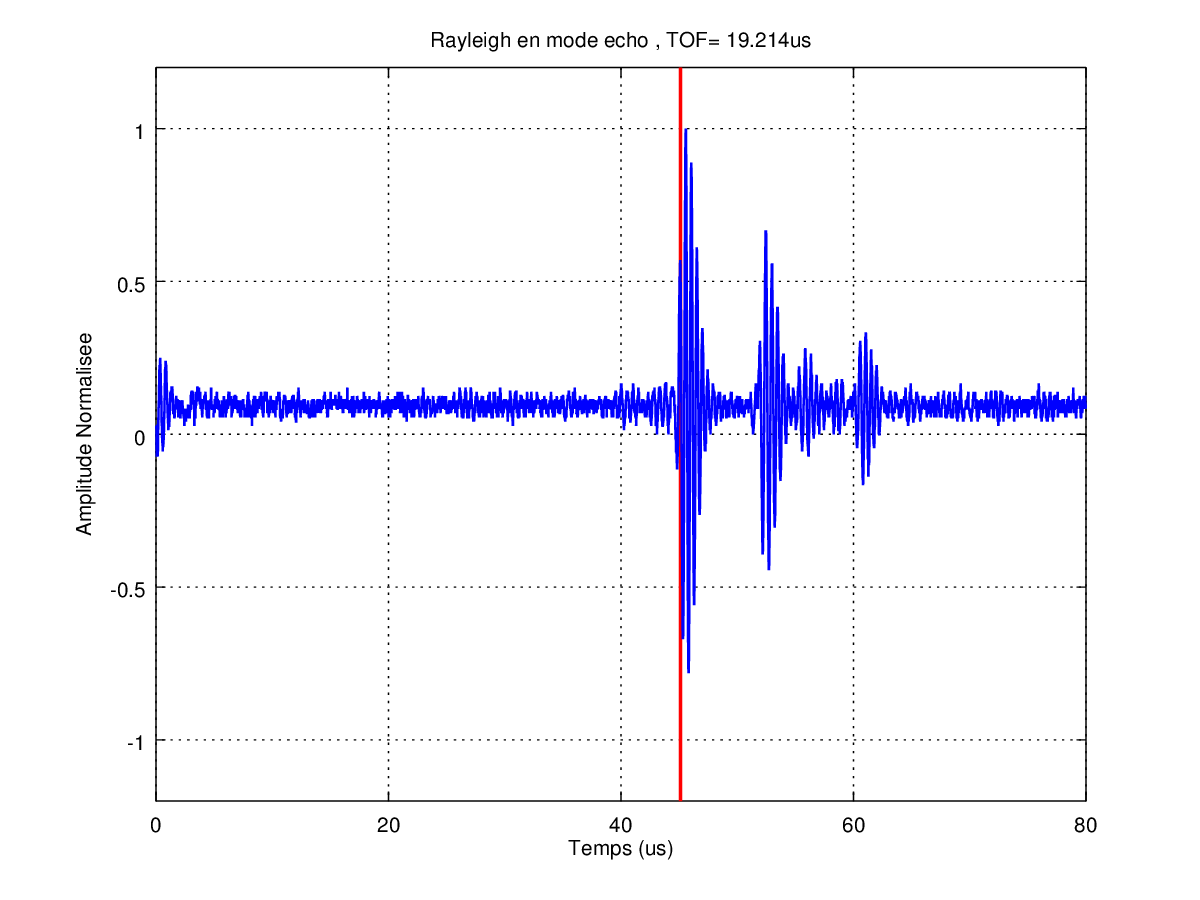
\includegraphics[width=.5\textwidth]{volsurf_figs/DS0008_rayleigh_echo.png}
    \caption{Mesure en mode écho de la vitesse des ondes de Rayleigh. la chaîne d'acquisition est paramétrée de sorte que le signal de synchronisation soit en $t=0$. Le front d'onde utilisé pour la mesure de vitesse est noté en rouge.}
    \label{volsurf:echo_norm}
\end{figurehere}

La valeur de vitesse précédente présente un écart relatif d'environ 2\% avec la valeur proposée par la solution de Viktorov (équation~\eqref{volsurf:an_viktorov}).

\subsection{Onde de surface et charge}

Les ondes de surface se propagent, comme leur nom l'indique, le long de l'interface et sont donc très sensibles à un changement de conditions limites.

Un cas bien connu est la génération d'ondes de Rayleigh généralisées mais un cas beaucoup plus simple consiste à venir poser une masse sur le trajet des ondes. Dès lors que la surface n'est plus libre, l'amplitude des ondes de Rayleigh est très fortement diminuée.

\section{Onde de Rayleigh généralisée}

Lorsque le fluide est visqueux ou simplement lorsque le couplage fluide-structure ne peut plus être négligé, il est coutume de parler d'onde de Rayleigh généralisée ou d'onde de Rayleigh de fuite\footnote{\textit{Leaky Rayleigh Wave} en anglais}. Ce nom vient du re-rayonnement d'énergie observable dans le fluide («\,fuite\,» d'énergie).

\begin{figure}
    \centering
    \begin{tikzpicture}[>=stealth]
        \draw[thick] (-3,1) -- ++(6,0);
        \draw[thick] (-3,2) -- ++(6,0);
        
        \draw[<-] (-2,2) -- ++(160:1) node[above] {$k_I$};
        \draw[dashed] (-2,1.5) -- ++(0,2);
        \draw (-2,2.5) arc (90:160:.5) node[midway,above] {$\theta_R$};
        
        
        \renewcommand\reray[1]{
            \draw[->] (#1,2) -- ++(20:1) node[above];
        }
        \reray{.5};
        \reray{1};
        \reray{1.5};
        \reray{2};
        
        \draw[dashed] (.5,2) -- ++(0,1);
        \draw (.5,2.5) arc (90:20:.5) node[midway,above] {$\theta_R$};
        \draw[->] (-1.5,1.7) .. controls (-1,2) and (-1,1.4) .. (-.5,1.7);
        
        \node at (1.7,3.2) {Re-rayonnement};
    \end{tikzpicture}
    \caption{Phénomène de re-rayonnement d'une onde de Rayleigh dans le fluide avoisinant.}
    \label{fig:my_label}
\end{figure}

Afin d'observer ce re-rayonnement, un montage en transmission latérale est mis en place.
Le transducteur émetteur, réglé pour un angle d'incidence correspondant à $\theta_R$ génère à la surface de la plaque une onde de Rayleigh.
De l'eau est placée sur le trajet de l'onde afin de faciliter le re-rayonnement et sa mesure.
Un transducteur est maintenu à la surface de l'eau (sans qu'il ne soit en contact avec la plaque).

La faible amplitude du re-rayonnement rend inutile la présentation ici de la trace mesurée, mais ce qui est essentiel, c'est qu'un re-rayonnement est bel et bien observé.
Les ondes de Rayleigh, identifiables à l'oscilloscope sont présentes dans la plaque et rayonnent dans le fluide. 

\section*{Conclusion}

Cette séance de travaux pratiques a été l'occasion de mieux comprendre les phénomènes de propagation en surface et dans le volume.
La mise en relation des connaissances théoriques sur les différents types d'onde avec les phénomènes observés a permis de mieux saisir les enjeux de la génération d'ondes de Rayleigh.
